\documentclass[titlepage, a4paper, 11pt]{scrartcl}

%too much whitespace otherwise
\usepackage[left=2cm,right=2cm,top=2cm,bottom=2cm]{geometry}

% Grafik Pakete
\usepackage{graphicx,hyperref,amssymb}

% Ordner für Grafiken
\graphicspath{ {./images/} }
\usepackage{float}

\usepackage[utf8]{inputenc}
\usepackage{amsmath}
\usepackage{amsfonts}
\usepackage{amssymb}
\usepackage{graphicx}

\usepackage{caption}
\usepackage{subcaption}

% Header and Footer
\usepackage{fancyhdr}

%bibtex
\usepackage{cite}
\usepackage{csquotes}

%code snippets
\usepackage{listings}
\usepackage{color}

\definecolor{dkgreen}{rgb}{0,0.6,0}
\definecolor{gray}{rgb}{0.5,0.5,0.5}
\definecolor{mauve}{rgb}{0.58,0,0.82}

\lstset{frame=tb,
    language=HTML,
    aboveskip=3mm,
    belowskip=3mm,
    showstringspaces=false,
    columns=flexible,
    basicstyle={\small\ttfamily},
    numbers=none,
    numberstyle=\tiny\color{gray},
    keywordstyle=\color{blue},
    commentstyle=\color{dkgreen},
    stringstyle=\color{mauve},
    breaklines=true,
    breakatwhitespace=true,
    tabsize=3
}

%dynamic image scaling
\newcommand{\imgScale}{0.7}

\pagestyle{fancy}
\fancyhf{}
\rhead{Julius Neudecker, 2025850, Page  \thepage}
\lhead{CEPH Cluster in containers}

%page numbering
\pagenumbering{arabic}

\title{Running a CEPH-Cluster from a containerized infrastructure}
\subtitle{Performance test with a mySQL-Database}
\author{Julius Neudecker \\ Bachelor of Science \\ \href{mailto:julius.neudecker@haw-hamburg.de}{julius.neudecker@haw-hamburg.de}}
\date{May 2021}


\begin{document}

    \maketitle

    \tableofcontents

    \begin{abstract}

        Setting up and operating a storage cluster with high availability is a complex task. 
        By using containerization, it is possible to abstract away and encapsulate some repetitive tasks.
        Therefore this study aims to analyse the possibility, implications and findings of a multi host
        CEPH-Cluster, where the individual daemons are entirely running within a containerized environment.
        To put the findings into a frame of reference, this study utilizes a mySQL-database which has 
        special requirements on data storage. The key points in terms of advantages and disadvantages,
        data integrity, performance and administion are scrutinized. Major findings are that there is a performace penalty which can be alleviated by optimizing the cluster configuration. However, these findings in the context of this paper are sometimes theoretical in nature since some constraints of the experimental environment had a significant impact on the results of the study.

    \end{abstract}

    \section{Introduction}

        In times where information is a valuable asset, it is of paramount importance to have a scalable and reliable
        way of storing data and information. Considerations about data throughput and 
        IOPS\footnote{Input/Output Operations per Second} are also a major design parameter on modern storage solutions.
        These different storage solutions provide different approaches on these considerations. For any given use case, there
        exist several options to adress these. Depending on the architecture and scope of the problem some are better
        suited than others. A few major considerations are apart from scalability, reliability and speed also cost effectiveness,
        vendor lock-in, complexity and granular customizability.

        Generally hardware based solutions have advantages in terms of raw performance but they often have significant disadvantages
        when it comes to vendor lock-in, easy scalability or restoration of corrupted disks. Software and network based solutions are
        usually less performant due to the network overhead. However this can be mitigated for the most part by scaling horizontally.

        Apart from proprietary cloud storage providers like AWS, Azure or Google, the open source community
        is heavily dominated by CEPH by more than twice as much as the next competitor:

        \begin{figure}[H]
            \centering
            \fbox{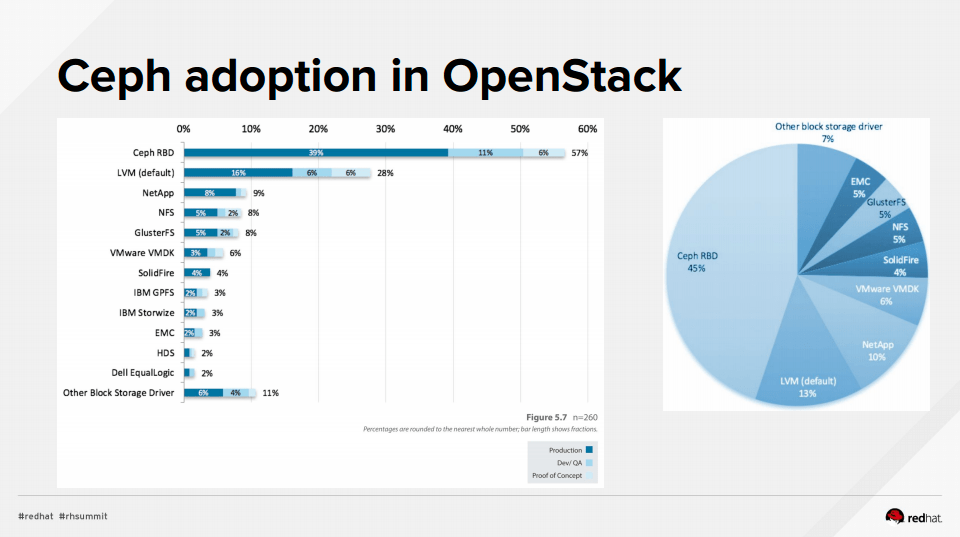
\includegraphics[width=\imgScale\textwidth]{marketshareCeph.png}}
            \caption{Adoption of CEPH in OpenStack in 2016, \cite{cephadoption}}
            \label{fig:ceph-market-share}
        \end{figure}

        Being conceived by Sage Weil for his doctoral thesis\cite{weil2007ceph}, CEPH became part of the Linux Kernel in 2010 and was acquired
        by RedHat in 2014, CEPH is gaining popularity steadily since its introduction as figure \ref*{fig:ceph-market-share} aims to show.

        Another modern important concept which is increasingly shaping modern technology stacks is \textit{OS level virtualization} or
        \textit{containerization} as its colloquially called. This way of deploying applications and services decreased the complexity of deploying several services and application on any given host dramatically by removing confliciting components and other means.

        Lastly, no storage solution exists without its use case. One major application, which requires flexible scaling are databases. 
        Scaling up databases is not an easy task as the tech stack is fairly monolithical in nature. A transparent, performant and scaleable storage solution would alleviate many problems.

        \subsection{Problem domains}\label{introduction}
            
            Managing a highly available storage cluster is not a trivial task. Apart from provisioning and monitoring the hardware,
            setting up multiple systems concurrently is a daunting task. Nowadays with infrastructure automation tools like Salt, Chef or Puppet, 
            this is easier than ever. However, it can still be a tedious task to tweak the configuration of these tools
            in order to make it work on a complex or diverse infrastructure. Especially in times when upates and EOL\footnote{End Of Life} events
            create incompatibilites between working application stacks on any given host machine.

            As for CEPH, this is especially true, since there are three major versions in production\cite{cephreleases}, as of Q1 2021.
            Deprecated features and bugfixes create functional inconsistencies between major versions, hence it is a necessity to 
            keep a cluster in production up to date. This necessitates constant modification and testing of the previously mentioned automation tools.

            One way to isolate these problems is \textit{OS Level Virtualization}. By doing so, every application or application stack 
            exists within a so called \textit{Container} and is therefore isolated from the host to a certain degree. 
            One inherent issue in this context is that they are stateless and ephemeral. This means that they can 
            \textit{by principle} be created and deleted according to momentary requirements. This process can be fully automated 
            \textit{orchestration software}. Therefore the virtualized production environment has to be
            configured in a way that allows it to provide the stability which is required for a storage engine.

            Trying to overcome the difficulties in setting up and manage a CEPH cluster with containerization might seem contradicting
            at first sight. The following sections focus on the major problem and adresses these. There are many related topics such as
            further optimizations for one or another particular use case. To adress these would go beyond the scope of this paper.
            Nevertheless a brief outlook on further considerations will be provided at the end in chapter \ref*{performance:tuning}.

        \subsection{Definition of research goal}\label{research-goal}
        
            The goal of this study is to evaluate if setting up a CEPH-storage cluster with containers is possible and if so, 
            if it is a feasable option for a production environment. In order to make a conclusive assessment, three main points 
            have to be examined:

            \paragraph{Data Integrity}

                This means running a service on the cluster, which is very sensitive to data inconsistencies.
                In this particular example a mySQL database is chosen. Databases have some unique properties, which makes them more sensitive 
                to issues with data replication and keeping clustered storages in sync. 
                Therefore this use case is chosen as a suitable real world application.

            \paragraph{Performance}

                Since performance is a main consideration in production environments, this is 
                the second most important key point. Depending on the overall cost structure of the environment, 
                a performance penalty might outweigh the benefits. In that case a containerized cluster 
                would be \textit{technically} possible but not economically feasable. Depending on the use case
                the important metric also differs. Fileserving services like storage clouds or streaming services 
                rely more on raw throughput. The data traffic with databases is generally rather small, therefore
                IOPS\footnote{Input/Output Operations per Seconds} are more important.

            \paragraph{Administration}

                One important reason to do reasearch in this topic is to evaluate if the time and effort to
                set up a cluster brings benefits in terms of administrative expenditure. At first sight a viable
                metric could be the spent time from starting to have a cluster up and running. However, depending
                on the production environment the results may vary to a wide degree. Therefore chapter \ref*{conclusion}
                will provide insight in the process of setting up this cluster and its problems and pitfalls.


        \subsection{Related Work}
        
            Since containerization and CEPH are already well established technologies, this section gives a brief overview of 
            other research which was already conducted in this area.
            RedHat in cooperation with Percona and Supermicro already conducted extensive research wheter it is feasable to
            run a SQL-Database on a CEPH-Cluster\cite{redhatstudy}. They concluded that indeed running a database on an 
            optimized CEPH-cluster exceeds industry standard database solutions. Furthermore scaling horizontally 
            is easier with a CEPH Cluster. Nevertheless it should be mentioned, that in this study the Percona 
            SQL distribution was utilized, which provides a native interface for kernel based RBD\footnote{Replicated Block Devices}.
            
            Hong et.al. used CEPH to create a framework which aims to mitigate handling issues with database containers.
            This includes the issues mentioned in chapter \ref*{introduction} that containers aren't persistent ways
            to store data\cite{hong2019database}. However this paper does not host the whole database container on a CEPH-cluster but only the volume to store the database tables and has therefore only little relevante to this topic.
            
            Although there are numerous other papers
            which discuss the process of setting up CEPH itself or in the context of an OpenStack environment,
            none of them discussed a similar scope as this.            

    \section{Setting up CEPH on Docker}

        This section is about setting up CEPH with containerization. Firstly, an extensive insight into CEPH and its underlying
        structure is provided. Secondly The system architecture for the experiments in the scope of this study is explained.
        This second section will make a small detour into containerization such as what it means, what the benefits and what the drawbacks are.

        \subsubsection{Containerization}\label{system:containerization}

            Although in the previous text the term containerization was mentioned a few times already, there was no
            definitive explanation as of what a container is or what containerization means. Firstly it is important to establish
            that containers are not \textit{something like} a virtual machine. In fact virtual machines are entire systems 
            which are executed on the hosts hypervisor\footnote{An abstraction layer for hardware and operating systems} and entirely self contained.
            This approach is really useful to deploy and maintain infrastructure since a machine with a defined behaviour can be
            launched in little time with no effort. However in the domain of application development or microservices especially with CI/CD\footnote{Continuous Integration/Continuous Deployment} pipelines in mind, this is an uneccessary overhead.
            Containers on the other hand are small entities, which contain only the neccessary components of an application or service to run and still have some degree of encapsulation to the host system.

            \begin{figure}[H]
                \centering
                \fbox{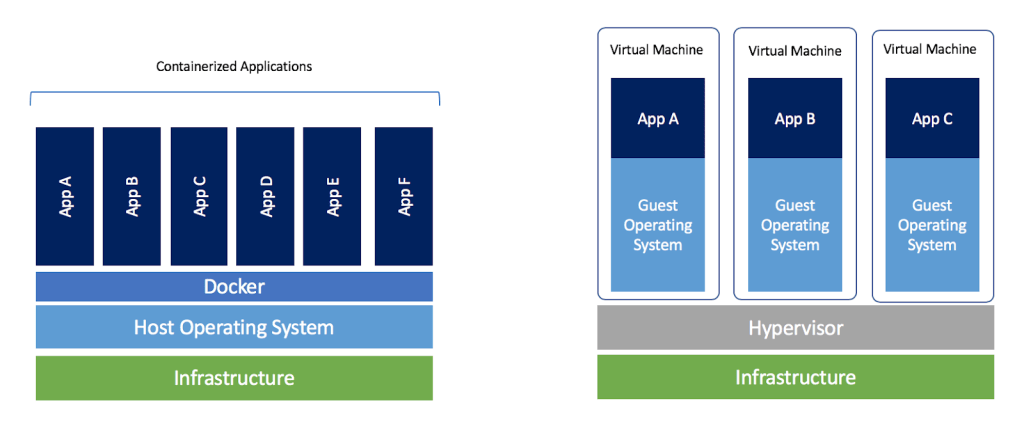
\includegraphics[width=\imgScale\textwidth]{docker-vs-vm.png}}
                \caption{Containerization compared to Virtualization, \cite{2021_docker}}
                \label{fig:docker-vs-vm}
            \end{figure}     

            By deploying applications or services this way, confliciting software versions, 
            applications and configurations can be encapsulated and thus solved. This makes scaling also easier, since scaling doesn't
            have to happen on a virtual machine level, which might cause additional costs for licensing, 
            services can be scaled on a more granular basis with containers and orchestration tools like
            \textit{Docker Swarm} or \textit{Kubernetes}, which will be explained in detail in section \ref{system:containerization}.
            As of Q1 2021, there exists a vast variety of different containerization solutions such as 
            Rkt, LXD and Docker\cite{cncf}. However Docker is unarguably the biggest solution in terms of 
            adoption, available images\footnote{Docker images are the blueprints to start containers from} and community.

        \subsection{CEPH Architecture}\label{ceph:arch}

            In short CEPH is a distributed solution for storage clusters. On one side it is specifically tailored to provide
            maximum reliability by distributing data over different disks, machines or even datacenters and therefore also 
            improving overall scalability and performance. On the other side it is also a cost effective solution because it is open source\cite{GitHubceph}
            and runs on commodity hardware. 

            The general structure includes several services which manage different functions within the cluster. In the context of
            CEPH these are called deamons, which are discussed in detail in the following sections.

            \begin{figure}[H]
                \centering
                \fbox{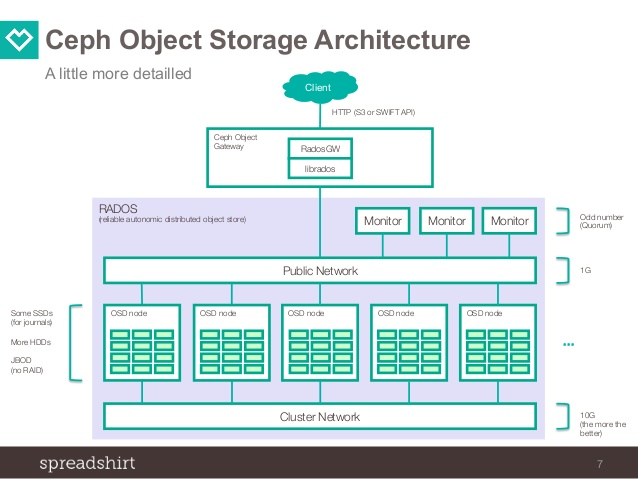
\includegraphics[width=\imgScale\textwidth]{ceph-architecture.jpg}}
                \caption{CEPH Architecture, \cite{hadlich_2015}}
                \label{fig:ceph-arch}
            \end{figure}
            
            Because it is a distributed system and may span over several physical machines, racks or even datacenters, inter-daemon
            communication plays a key role. For the purpose of autonomous data replication the cluster relies on a dedicated network.
            This network is separated from the public network, which is for client data access. Figure \ref{fig:ceph-arch} provides a 
            general overview.

            How the data is distributed internally is determined by two main factors: \textit{Placement Groups} and the \textit{CRUSH} algorithm.
            Placement Groups (abbreviated \textit{PG}) is CEPHs way to keep track of the physical location of objects.
            Files are split up into different objects, where each object is stored in a different PG, which is determined by the 
            CRUSH\footnote{Controlled, Scalable, Decentralized Placement of Replicated Data} algorithm\cite{weil2007ceph}. Figure \ref{fig:ceph-crush}
            shows a schema of how this works.
            The reasoning behind PGs is that keeping track of millions of objects via metadata is computationally expensive\cite{PGcephDocu}.
            Therefore objects are hashed and assigned to PGs.
            A so called CRUSH-Map keeps track of the structure of the whole cluster. This will become important in section \ref{system:crush-fail}.

            \subsubsection{Cluster Access}

                To access the cluster CEPH provides different interfaces depending on the use-case:

                \begin{itemize}
                    \item \textit{CephFS} - A POSIX\footnote{Portable Operating System Interface - Part of the Unix specification} conform filesystem
                    \item \textit{LIBRBD/KRBD} - A block device
                    \item \textit{RADOSGW} - An REST gateway for storage buckets
                    \item \textit{LIBRADOS} - The API to access the cluster directly from applications
                \end{itemize}

                All these interfaces are based on LIBRADOS, provides the interface to access RADOS. This is the underlying object store
                responsible for distributing the data over several phsyical disks. This task is done by the \textit{OSD}-Daemon.

                \paragraph{CephFS} is the filesystem, which allows for CEPH to behave to the user or the operating system like any other
                filesystem would. However is has to be distinguished from from a block device. 
                The key is that it is not a filesystem like EXT4 or NTFS. It is more a translation layer to the
                RADOS\footnote{Reliable Autonomous Distributed Object Storage} interface. A required metadata service called \textit{MDS} provides journaling functionality and handles client access. Because the throughput of the whole cluster scales linearly with the size of the cluster,
                several different MDSs are required on big clusters to handle the client load and distribute the file metadata. Thus also mitigating
                single points of failure. It is best practice to store and serve the MDS from fast solid state drives to reduce hardware bottlenecks.

                \paragraph{LIBRBD/KRBD} is a virtual block device. The difference to CephFS is that is behaves like a physical disk.
                Therefore it can be formatted with any filesystem like EXT4 or NTFS. The distinction between \textit{LIB}RBD and \textit{K}RBD
                means userspace for LIBRBD and kernelspace for KRBD. To explain these differences between these two would go beyond the 
                scope of this paper and requires knowledge about kernels, operating systems and memory handling. 

                \paragraph{RADOSGW} provides as REST gateway access to S3\footnote{Simple Storage Service} buckets. Unlike filesystems or block devices, these S3
                buckets don't have a hierarchical structure with directories. All objects are stored on the same level, therefore the 
                analogy to a bucket. This bucket is addressed by means of an API which provides also a metadata filter to select
                specific files directly.
                A widely adopted use case is serving static files on the internet for media content, javascript or css files by content delivery networks.
                They can also be used to store virtual disk images to be used in conjunction with RBDs to name a few use cases.

                \paragraph{LIBRADOS} provides a native API to access RADOS directly without any file system or block device translation layer in
                between. The higher development costs for a more complex implementation might be worth the gains in throughput and IOPS
                for critical applications. This is implemented in the Percona mySQL Server\cite{redhatstudy}.

            \subsubsection{Object Storage Devices - OSD}

                Within the CEPH domain, these are the disks, where the actual data objects are stored to. 
                One or more OSDs can be handled from one CEPH OSD Daemon, which provides the connecting layer to the whole cluster.
                Also one OSD can contain several PGs. This depends on the configuration of the cluster. On which disk and in which PG
                and object is stored is determined by the CRUSH algorithm as shown in figure \ref{fig:ceph-crush}.
                Since data is replicated within the cluster and constantly updated, one OSD could fail and the data and PGs of this failed
                OSD will be written to another OSD. This constant data shuffling takes place transparent to the user and is the reason why CEPH
                needs a dedicated network as mentioned in section \ref{ceph:arch}. How the data is physically stored on the disk differs between
                the two different backends used in older or newer releases: Bluestore and Filestore. Where Bluestore is the newer and more performant standard.
            
            \subsubsection{Monitor Nodes - MON}

                Monitor Nodes (abbreviated as \textit{MON}) have two main purposes: They maintain a copy of the cluster map to hand this out 
                to a client, which connects to the cluster. Because of a fault in a MON this map might not reflect the state of the cluster accurately.
                Therefore an odd number of MON nodes have to reach a quorum on the current state of the cluster and distribute the correct cluster map.
                According to the CEPH documentation this is negotiated via the \textit{PAXOS} algorithm\cite{MONcephDocu}.
                Although a cluster could technically work with just one MON node, it is highly recommended to have at least three MON nodes,
                removing a single point of failure.

                \begin{figure}[H]
                    \centering
                    \fbox{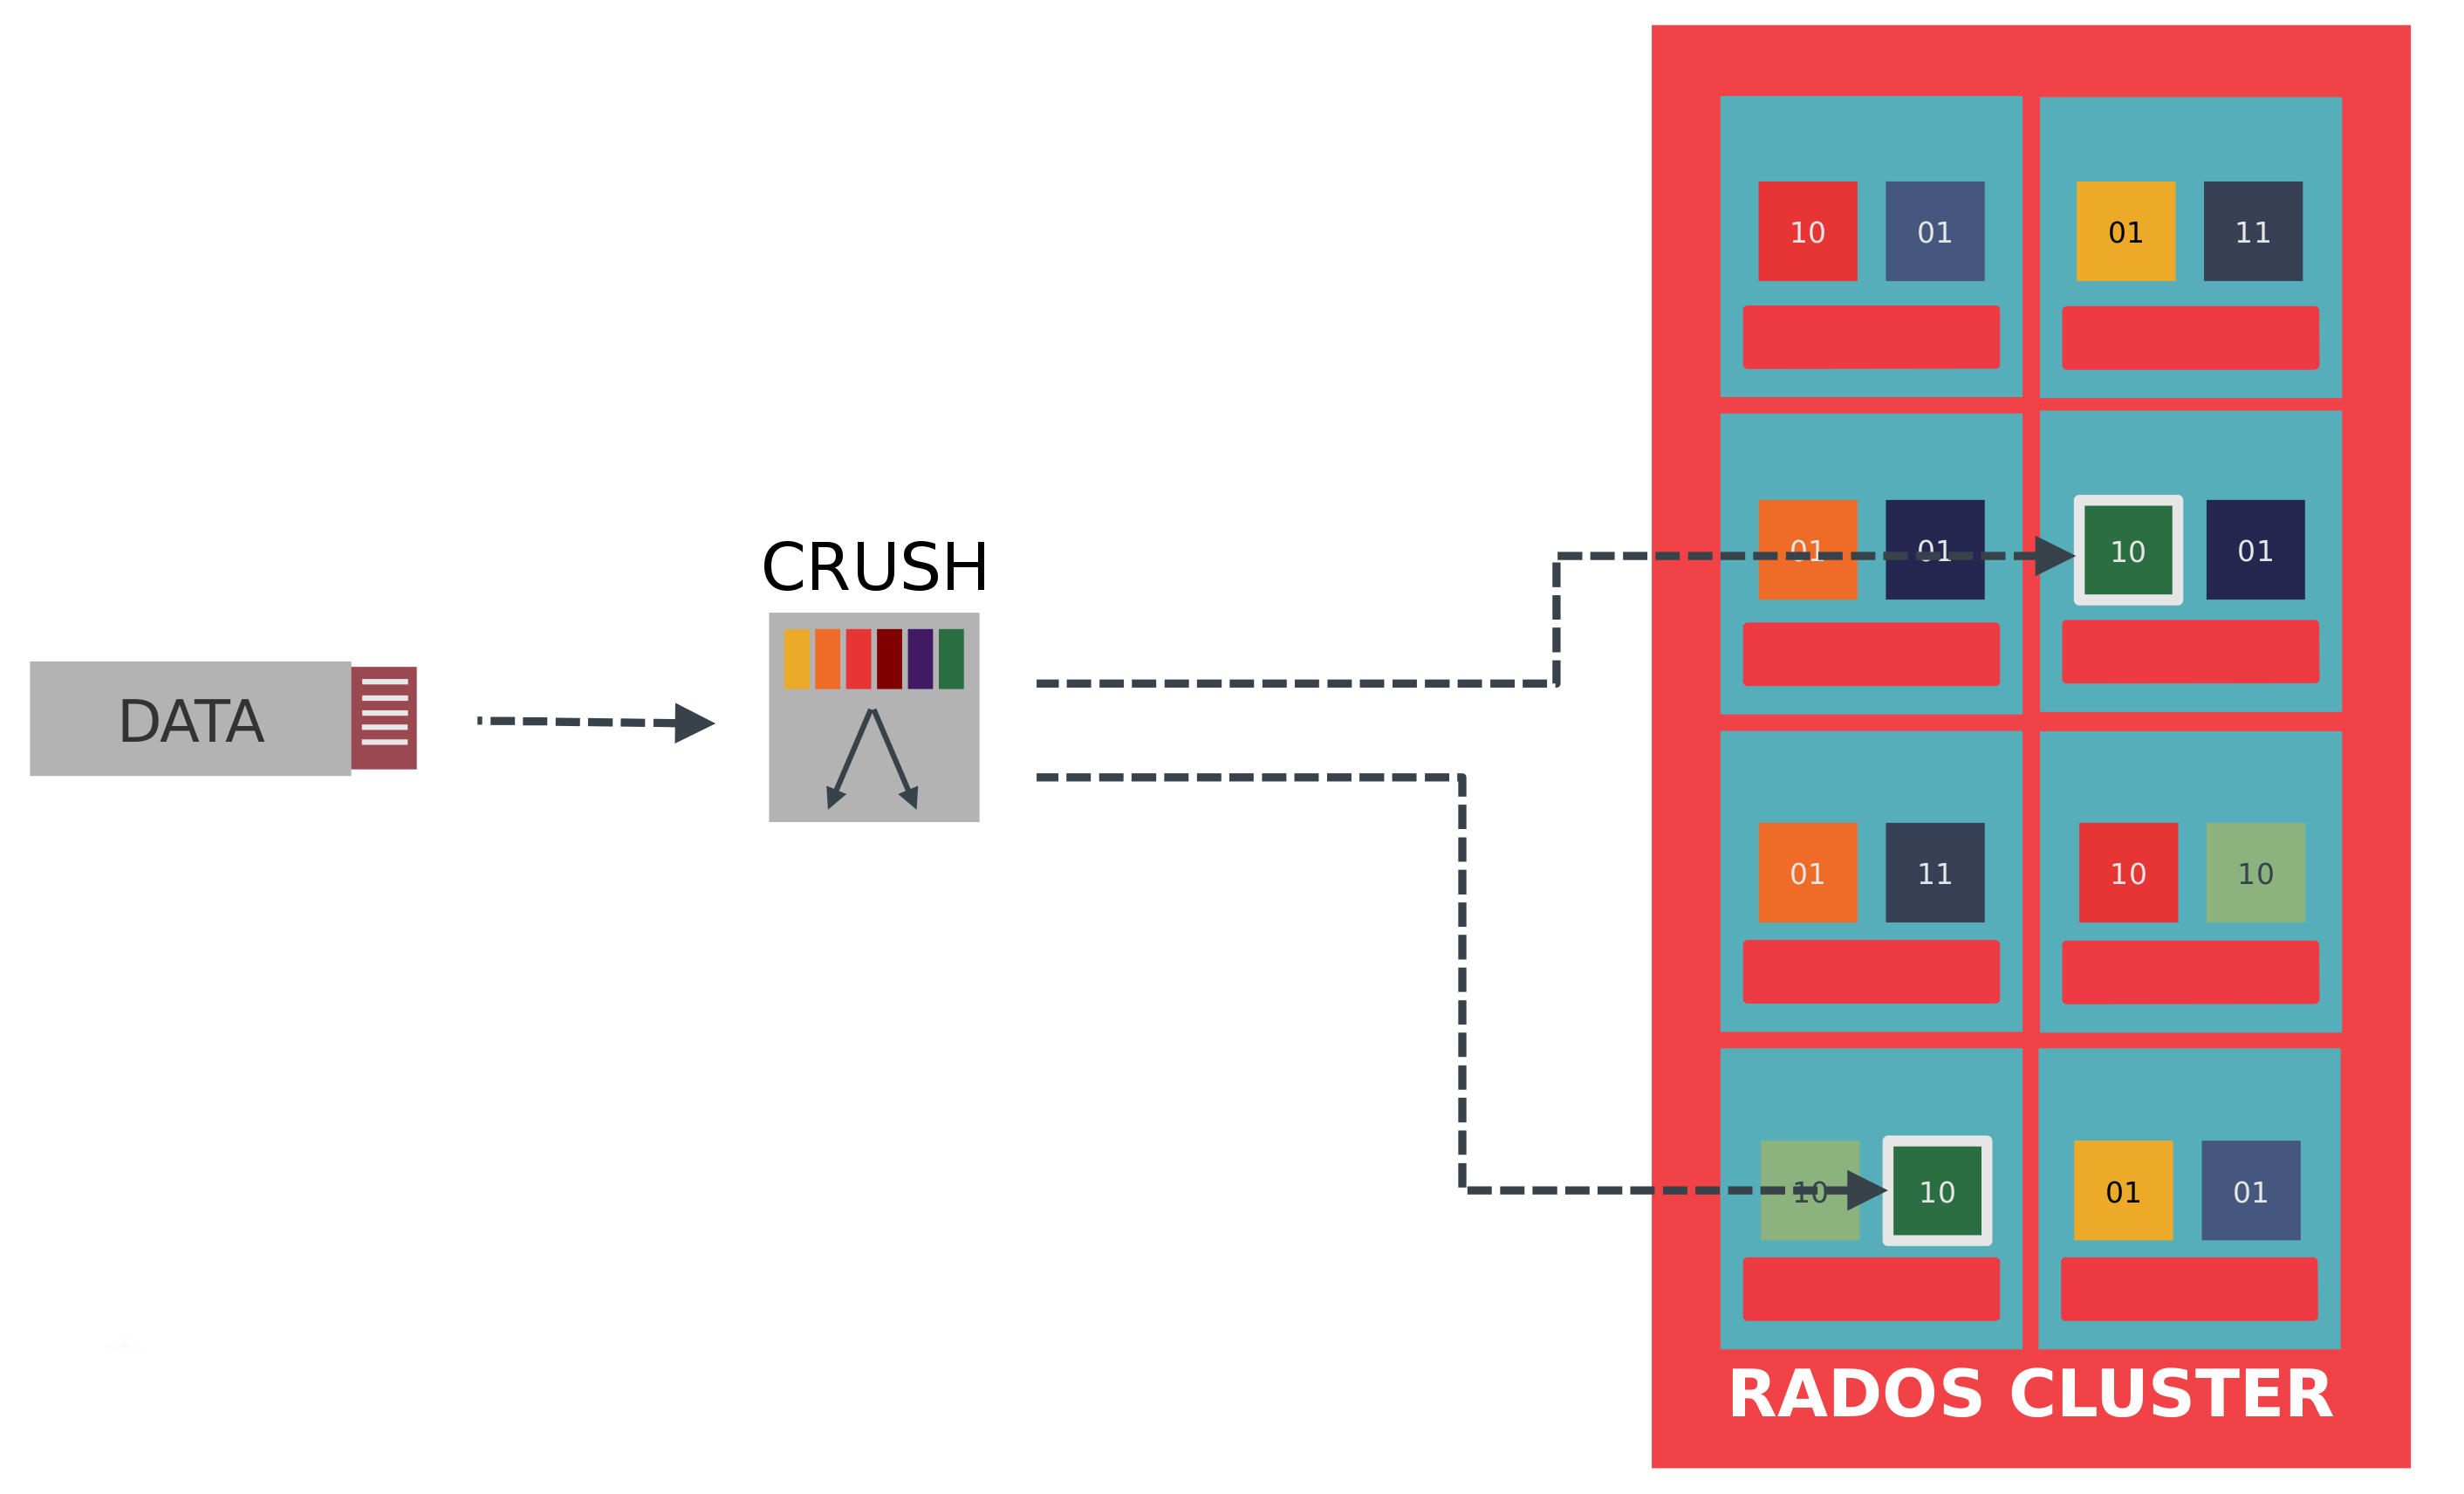
\includegraphics[width=\imgScale\textwidth]{Ceph-crush-map.png}}
                    \caption{Placement Groups and CRUSH Algorithm, \cite{krenn2020}}
                    \label{fig:ceph-crush}
                \end{figure}                           

            \subsubsection{Metadata Server - MDS}

                The metadata server is not neccessary for the cluster to operate as RBD, storage bucket or via Librados API.
                However to provide a journaled filesystem via the CephFS, this service is needed to provide the filesystem metadata such
                as permissions and timestamps. As stated from RedHat, it is best practice to deploy a MDS with big and fast nVME drives\cite{redhatstudy}.
                These can be also used in conjunction with memcached, where the recent metadata are stored into the RAM of the MDS.
                Overprovisioning, automatic failover and scalability are the main considerations for MDS to have high availability and high performance.

            \subsubsection{Manager - MGR}   
            
                Since the 12.x release, CEPH needs a manager node to operate\cite{MGRcephDocu}. This manager does not provide any
                functionality to the cluster itself but acts as an interface to external monitoring tools and systems. Without it 
                the state of the cluster won't appear to be healthy nor be externally visibly updated\cite{MGRcephDocu}.              

        \subsection{System Architecture}\label{system:my-setup}

            In this section I'll go over the system architecture in my experiments since its understanding is vital to the understanding
            of the configuration of the containers later on.

            Firstly, because of the Covid-19 pandemic I couldn't use the lab in the university so I had to rely on my personal ressources 
            in order to do my experiments. Since these are somewhat limited I configured a few things different than it would be usually done.

            \textit{I assume that the reader has a basic understanding of Docker and how commands are executed or how containers work in detail. Therefore topics which are immaterial to this topic won't be explained in great detail.}

            \subsubsection{Hardware Diagram}

                The cluster is distributed across three different machines for storage. Since the latest CEPH version isn't available as Docker Image for ARMv7 and ARMv8 architectures, the only available x86\_64 host acts as Docker host for all containers including the OSDs. 
                However to create constraints such as network latency and bandwith, the physical volumes were
                attached to the ARM-Machines and mounted as iSCSI devices on the Docker host. Because in this small setup the available CPU performance and RAM is not a concern, running a few more containers isn't a big concern. 

                \begin{figure}[H]
                    \centering
                    \fbox{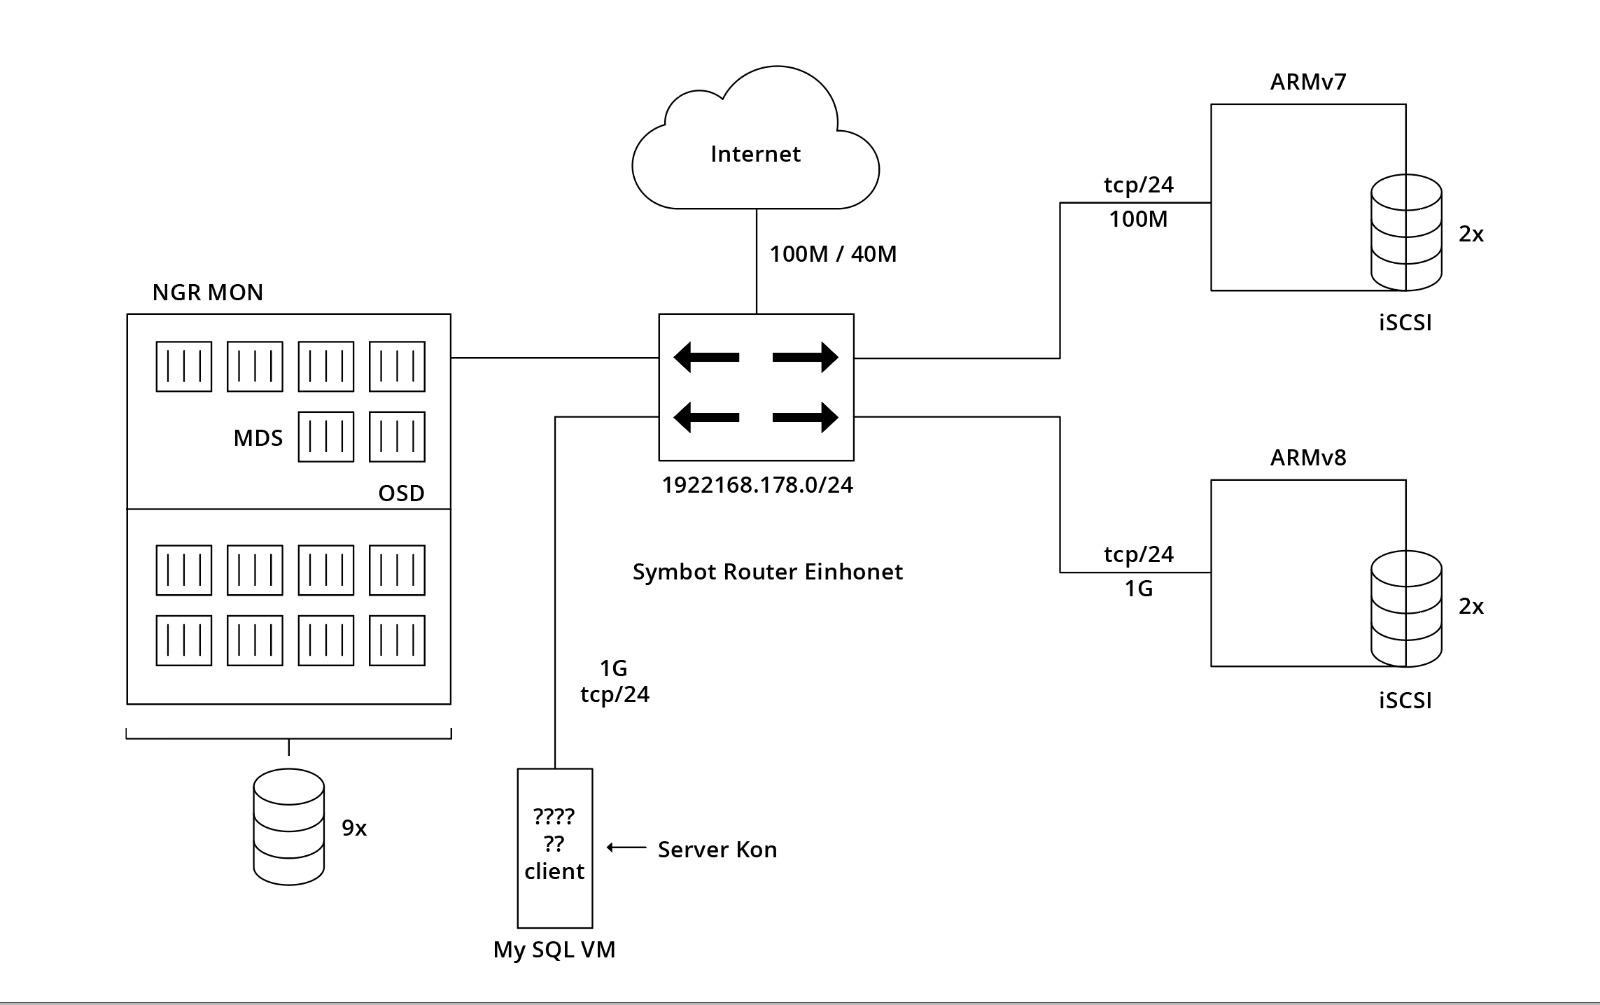
\includegraphics[width=\imgScale\textwidth]{architecture.jpeg}}
                    \caption{Hardware Diagram}
                    \label{fig:hardware-diagram}
                \end{figure}   

                Furthermore the Docker host is a server in production for serving websites and services. 
                Therefore a certain amount of system ressources were already allocated to other running processes.
                Since my tests were exclusively conducted in the local network, the bandwith of the internet connection wasn't a concern either.
                Usually a CEPH cluster uses two seperate networks: one for replicating data between the OSDs and one to client access to the cluster or configuration.
                In this case only one physical network was available, which has a bandwith of 1GBit/s

            \subsubsection{Docker Config for CEPH Image}\label{config:docker}

                By starting CEPH as a container, a lot of configuration work is abstracted away already in the Docker image.
                The official image \cite{DockerHub} provides two options to distribute the configuration between the different nodes:

                \begin{itemize}
                    \item On disk
                    \item KV-Store\footnote{As of Q1 2021 only etcd is supported by the official image}
                \end{itemize}

                The same Image provides all the different daemons, which are needed in a CEPH cluster and thus every container is configured different.
                The configuration is stored \textit{on Disk} because all containers are executed on the same physical host, hence a remote KV-Store isn't required.
                This is reflected by the two directories \textit{/docker/ceph/data/etc/} and \textit{/docker/ceph/data/lib}, which all containers have in common.
                
                Another issue is that the MON and OSD nodes run into timeout issues, when deployed on the same host and configured to use Dockers \textit{--net=host} option, as suggested by the official manual. This would effectively bind the ports of any container, which is configured in that way, directly to the host interface. 
                I chose another approach: providing each container with a dedicated IP-Adress within the network. This is possible by using the \textit{MACVLAN} network
                driver which is provided by the Docker engine. This allows every container which has this driver enabled to appear as a seperate host apart from the docker host. The IP is configured with the \textit{--ip=192.167.178.2XX} option.

                The complete configuration is made available under a repository \cite{ghceph}.

                \paragraph{Monitor Nodes}

                    The network configuration of the monitor nodes is of special interest here: The public network has to be configured in case there are two 
                    distinct networks as explained in \ref{ceph:arch}. This is not neccessary for the other nodes since the configuration will be distributed
                    after the monitor nodes are online.

                    \begin{lstlisting}
                        docker run -d \textbackslash
                        -v /docker/ceph/data/etc:/etc/ceph \textbackslash
                        -v /docker/ceph/data/lib:/var/lib/ceph/ \textbackslash
                        -e MON_IP=192.168.178.220 \textbackslash
                        -e CEPH_PUBLIC_NETWORK=192.168.178.0/24 \textbackslash
                        --ip=192.168.178.220 \textbackslash
                        --network=macvlan0 \textbackslash
                        --name ceph_mon1 ceph/daemon mon                        
                    \end{lstlisting}

                \paragraph{Manager Nodes}

                    This container runs in parallel to a monitor node and doesn't need any special configuration. For a healthy cluster only one node instance is required.

                    \begin{lstlisting}                    
                        docker run -d \textbackslash
                        -v /docker/ceph/data/etc:/etc/ceph \textbackslash
                        -v /docker/ceph/data/lib:/var/lib/ceph/ \textbackslash
                        --ip=192.168.178.223 \textbackslash
                        --network=macvlan0 \textbackslash
                        --name ceph_mgr ceph/daemon mgr
                    \end{lstlisting}

                \paragraph{OSD Nodes}

                    The configuration of the OSD nodes is more complicated compared to the other nodes. I chose to provide a physical disk
                    to the container. Therefore it had to be initialized as a logical volume before the OSD node is able to utilize it.
                    The official CEPH image provides a configuration option for this purpose. The following command creates a temporary container,
                    which is configured by the \textit{--rm} command. The \textit{--data /dev/sdX} command specifies the physical disk, which will be 
                    pre-treated. A prerequisite is that any disk has to be completely wiped of any partition table. This is done by executing \textit{sgdisk -xz}
                    prior to launching the preparation container on every drive to wipe out any existing partition table.

                    \begin{lstlisting}
                        docker run --rm \textbackslash
                        --privileged=true \textbackslash
                        -v /docker/ceph/data/lib:/var/lib/ceph/ \textbackslash
                        -v /var/log/ceph:/var/log/ceph/ \textbackslash
                        -v /docker/ceph/data/etc:/etc/ceph \textbackslash
                        -v /dev/:/dev/ \textbackslash
                        -v /run/lock/lvm:/run/lock/lvm:z \textbackslash
                        -v /run/lvm/:/run/lvm/ \textbackslash
                        -v /var/run/udev/:/var/run/udev/:z \textbackslash
                        --ip=192.168.178.230 \textbackslash
                        --network=macvlan0 \textbackslash
                        --entrypoint ceph-volume ceph/daemon lvm prepare \textbackslash
                        --bluestore \textbackslash
                        --data /dev/sdX \textbackslash
                        --no-systemd                            
                    \end{lstlisting} 

                    When the disk is prepared, it appears as \textit{lvm-partition} with a ceph-prefix. The OSD node can then be started by executing the following command:

                    \begin{lstlisting}
                        docker run -d \textbackslash
                        --privileged=true \textbackslash
                        --pid=host \textbackslash
                        -v /docker/ceph/data/etc:/etc/ceph \textbackslash
                        -v /docker/ceph/data/lib:/var/lib/ceph/ \textbackslash
                        -v /dev/:/dev/ \textbackslash
                        -v /run/udev/:/run/udev/ \textbackslash
                        -e OSD_DEVICE=/dev/sde \textbackslash
                        -e OSD_TYPE=disk \textbackslash
                        -e OSD_BLUESTORE=1 \textbackslash
                        -e CEPH_DAEMON=OSD_CEPH_VOLUME_ACTIVATE \textbackslash
                        -e OSD_ID=0 \textbackslash
                        --ip=192.168.178.230 \textbackslash
                        --network=macvlan0 \textbackslash
                        --name ceph_osd_sde ceph/daemon osd
                    \end{lstlisting}

                    There are some important things to consider here: firstly the \textit{--pid=host} configuration is neccessary to prevent that the host system
                    runs out of open file handles. This is a known bug, which is explained here on the Github page of the Docker Image \cite{cephdockerbug}. The 
                    \textit{--privileged=true} setting is neccessary to give the required access to disks from within the container. However from a security standpoint this is not good practice and should never be used in that way in a production environment! \textit{OSD\_BLUESTORE=1} configures the way CEPH stores the data in the background and \textit{OSD\_ID=X} defines the ID under which the OSD will be reffered to by the cluster.

                \paragraph{Metadata Nodes}

                    Since one phyisical host can host many different metadata nodes to provide peak performance, these MDS nodes have to be named uniquely. This is done 
                    by using the \textit{\$hostname-x} variable. Also the official image is recommending to set the \textit{CEPHFS\_CREATE=1} flag. On my setup however this resulted in an error and the filesystem was not being created. In my case I had to create the filesystem manually from within the monitor container by using the \textit{docker exec} command to open a terminal within the container. Therefore this flag has to be set to "0" in this case.

                    \begin{lstlisting}
                        docker run -d \textbackslash
                        -v /docker/ceph/data/lib:/var/lib/ceph/ \textbackslash
                        -v /docker/ceph/data/etc:/etc/ceph \textbackslash
                        -e CEPHFS_CREATE=0 \textbackslash
                        -e MDS_NAME=mds-$(hostname)-a \textbackslash
                        --ip=192.168.178.245 \textbackslash
                        --network=macvlan0 \textbackslash
                        --name ceph_mds_a ceph/daemon mds
                    \end{lstlisting}   
                    
            \subsubsection{CRUSH Fail mode}\label{system:crush-fail}

                In order to define the behaviour of the cluster in case of failures, CEPH provides a setting
                which is called \textit{CRUSH Fail Mode}. This setting defines the biggest possible failure domains, 
                which should not affect data integrity\cite{crushFailure}. In consequence, data is replicated in a
                way which guarantees this. To pick a few examples: 

                \paragraph{OSD (or device)} means that a single drive could fail and no data will be lost.
                This would be the preferred setting when the cluster runs on a single machine. However, if the cluster
                consists of more than one machine and the whole machine fails because of a PSU\footnote{Power Supplying Unit} failure
                for example, data integrity cannot be guaranteed anymore.

                \paragraph{Chassis} is the failure mode for rack mounted servers, where a multitude of servers
                make up the whole cluster. This would cover the previously mentioned case, which might be as well interesting for maintenance,
                when individual machines have to be maintained or being decommissioned.
                
                \paragraph{Rack} provides data integrity across multiple chassis or hosts on a datacenter level. If for example
                a critical component of the network infrastructure fails, this could provide some security. Although CEPH clusters 
                are in principle set up in a way which prevents SPOF\footnote{Single Point Of Failure}, this must not be true for the
                peripheral infrastructure. 

                \paragraph{Datacenter} usually means that a huge number of several racks, consisting of multiple chassis are grouped
                together as a common failure domain - in case of a power outage or natural disaster. If the company which owns the datacenter,
                operates on a global scale this failure mode is also a consideration for performance. Because of physical and network
                topology, the RTT\footnote{Round Trip Time} to a certain datacenter might be longer than desired. If all data is replicated
                on datacenter granularity, a global scale data integrity is guaranteed as well as the possibly shortest response time.

                \paragraph{In general} the failure mode should be as granular as possible but also as fine as financially feasable.
                In the context of the system architecture in the scope of this study (see section \ref{system:my-setup}), the fail mode will be on an OSD level.
                Because my experimental setup consists of multiple disks and flash storages with different ages and levels of degradation.
                However, the appropriate setting would be \textit{host}-level data replication.

            \subsubsection{Creating the cluster}

                Although there are different solutions to automate the deployment of a cluster such as \textit{CEPH-Ansible}\cite{cephansible} or \textit{CEPH for Rook}\cite{RookDocs} my cluster is rolled out and configured with a simple shellscript - \textit{startup.sh}\footnote{see Github repo for the whole document} - which creates a fully functional cluster:

                \begin{lstlisting}
                    #!/bin/sh

                    ## start MON and MGR
                    docker run -d -v /docker/ceph/data/etc:/etc/ceph -v /docker/ceph/data/lib:/var/lib/ceph/ -e MON_IP=192.168.178.220 -e CEPH_PUBLIC_NETWORK=192.168.178.0/24 --ip=192.168.178.220 --network=macvlan0 --name ceph_mon1 ceph/daemon mon
                    docker run -d -v /docker/ceph/data/etc:/etc/ceph -v /docker/ceph/data/lib:/var/lib/ceph/ --ip=192.168.178.223 --network=macvlan0 --name ceph_mgr ceph/daemon mgr

                    docker exec -it ceph_mon1 ceph auth get client.bootstrap-osd -o /var/lib/ceph/bootstrap-osd/ceph.keyring

                    ## prepare and create OSDs
                    ./prepare.sh
                    ./create.sh

                    ## create fs
                    docker exec -it ceph_mon1 ceph osd pool create cephfs_data
                    docker exec -it ceph_mon1 ceph osd pool create cephfs_metadata
                    docker exec -it ceph_mon1 ceph fs new cephfs cephfs_metadata cephfs_data

                    ##create the additional MON and MDS after the cluster has been created
                    docker run -d -v /docker/ceph/data/etc:/etc/ceph -v /docker/ceph/data/lib:/var/lib/ceph/ -e MON_IP=192.168.178.221 -e CEPH_PUBLIC_NETWORK=192.168.178.0/24 --ip=192.168.178.221 --network=macvlan0 --name ceph_mon2 ceph/daemon mon
                    docker run -d -v /docker/ceph/data/lib:/var/lib/ceph/ -v /docker/ceph/data/etc:/etc/ceph -e CEPHFS_CREATE=0 -e MDS_NAME=mds-$(hostname)-a --ip=192.168.178.245 --network=macvlan0 --name ceph_mds_a ceph/daemon mds

                    docker run -d -v /docker/ceph/data/etc:/etc/ceph -v /docker/ceph/data/lib:/var/lib/ceph/ -e MON_IP=192.168.178.222 -e CEPH_PUBLIC_NETWORK=192.168.178.0/24 --ip=192.168.178.222 --network=macvlan0 --name ceph_mon3 ceph/daemon mon
                    docker run -d -v /docker/ceph/data/lib:/var/lib/ceph/ -v /docker/ceph/data/etc:/etc/ceph -e CEPHFS_CREATE=0 -e MDS_NAME=mds-$(hostname)-b --ip=192.168.178.246 --network=macvlan0 --name ceph_mds_b ceph/daemon mds

                    exit 0
                \end{lstlisting}

                The docker run commands are the same as above but executed in a specific order. One monitor node has to be launched first to create an initial cluster configuration.
                Shortly thereafter follows a manager node. The next line deploys the keyring-file to the other bootstrap directories. Since all containers are deployed on a single machine, every node can access this keyring in its respective bootstrap directory. The script \textit{prepare.sh} and \textit{create.sh} executes the commands mentioned under the OSD part of section \ref*{config:docker} for each disk.
                The next strep is the creation of the filesystem. According to the docker documentation the FS will be created upon launch of the MDS node with the \textit{CEPHFS\_CREATE=1} parameter defined. However this didn't work properly in my case. The lines with \textit{docker exec ...} execute a command within the denominated container (in this case 
                \textit{ceph\_mon1}) from the host shell. These three commands create the data pools and the filesystem, which requires as metadata pool and a data pool \cite{CreateaCephfilesystem}.
                The following lines are only the additional MON and MDS nodes being created. These are not strictly neccessary for the cluster to function but provide redundancy to secure the \textit{no single point of failure} design of CEPH.

    \section{System Analysis}

        To measure the performance of the cluster, I chose to use two tools: \textit{scbench} and \textit{mysqlslap}. Both tools give detailed insight into
        the critical performances figures for such a cluster. As for the raw read/write performance test I can only evaluate the performance of the cluster at hand for reasons mentioned 
        in \ref*{system:my-setup}. However since my server has different storage technologies, I can evaluate the database performance with the cluster, an HDD and SSD.

        \subsection{SCBENCH} 

            % scbench: https://access.redhat.com/documentation/en-us/red_hat_ceph_storage/4/html/administration_guide/ceph-performance-benchmarking
        
            This tool measures the raw performance of a CEPH cluster by performing a write and subsequent read test sequential and random\textbf{REF TO REDHAT}.
            I performed three different tests with different loads on the cluster:

            \begin{itemize}
                \item 10 seconds with 16 threads
                \item 30 seconds with 32 threads
                \item 60 seconds with 64 threads
            \end{itemize}

            My goal is to load the cluster in a way that eventually all caches and short term performance enhancements become saturated to gauge the stable long term performance.
            What exactly scbench does under the hood, is described in great detail under \textbf{RESEARCH LINK}.

            This test yields three different performance parametres for read and write actions:

            \begin{itemize}
                \item Bandwidth
                \item IOPS
                \item Latency
            \end{itemize}

            For reading the test was executed for sequential and random access of the data. However the tests for sequential read access weren't sufficient enough to evaluate, therefore I will only show the results for random read, which is more important in the context of database operations anyway.

            \textit{All graphs were created from the raw data, which scbench provides. The code to reproduce these results is available under}\textit{[ADD REPOLINK]}

            \paragraph{Write performance}

                Before executing the read performance test, \textit{scbench} has to execute the write test in order to have readable data available.

                \begin{figure}[H]
                    \centering
                    \fbox{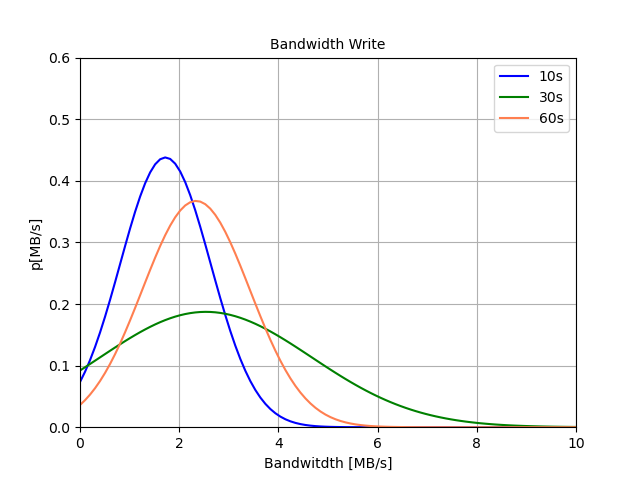
\includegraphics[width=\imgScale\textwidth]{Write_Bandwidth.png}}
                    \caption{Normal distribution of the writespeed for three different tests}
                    \label{fig:write-speed}
                \end{figure}   

                Figure\ref*{fig:write-speed} shows the saturation of the write speed with increasing load. On write operations with a short duration,
                the cost of the whole procedure of contacting the cluster to receive the correct endpoints to write to is relatively high, therefore the initial
                period where no data is written has an overall bigger impact on the measurement. As the client is writing more data to the OSDs, the writespeed increases.
                However after the different caching entities within the cluster become saturated, the writespeed eventually stabilizes at around 2.5MB/s.

                \begin{figure}[H]
                    \centering
                    \fbox{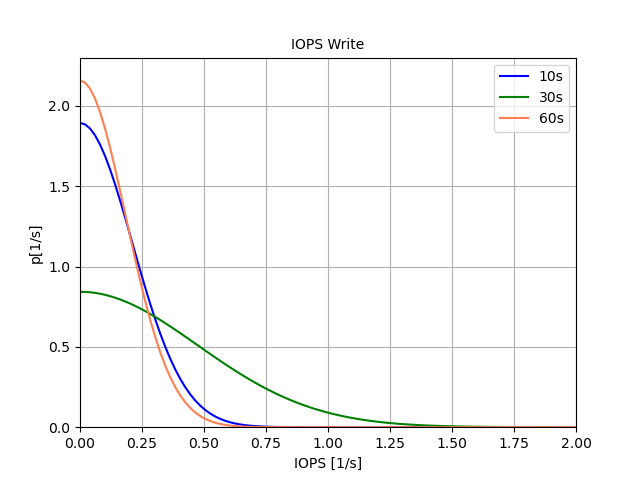
\includegraphics[width=\imgScale\textwidth]{Write_IOPS.png}}
                    \caption{Normal distribution of the write IOPS for three different tests}
                    \label{fig:write-iops}
                \end{figure}   

                The write IOPS in figure \ref*{fig:write-iops} exhibits the same result: Initial IOPS start slow due to the cost of initializing, subsequently increasing as the initialization has a smaller impact on the results but with saturation decreasing again. 

                \begin{figure}[H]
                    \centering
                    \fbox{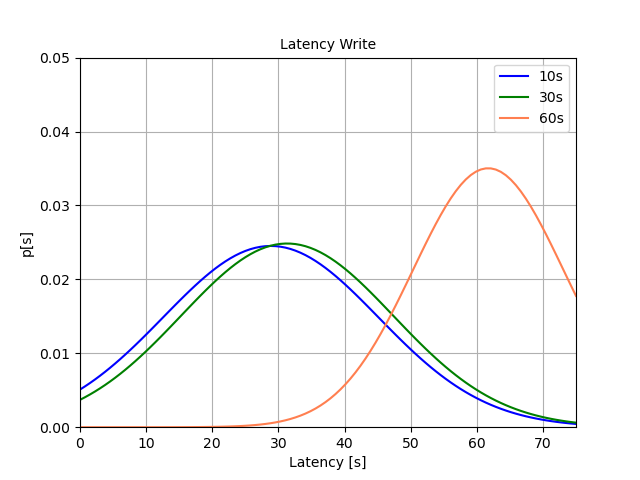
\includegraphics[width=\imgScale\textwidth]{Write_Latency.png}}
                    \caption{Normal distribution of the write latency for three different tests}
                    \label{fig:write-latency}
                \end{figure}   

                The write latency for the 10s and 30s mark shown in figure \ref*{fig:write-latency} is about the same. The saturated case after 60s however is an interesting anomaly. The best explanation is that the process of reorganizing data and placement groups takes away performance and therefore increasing latency.
                This is especially plausible since all data transactions are processed over the same physical network interface since this cluster does not have a dedicated network for this task\textbf{[INSERT NOTE TO SETUP HERE]}.

            \paragraph{Read performance}

                This test reads the previously created data during the write test randomly.

                \begin{figure}[H]
                    \centering
                    \fbox{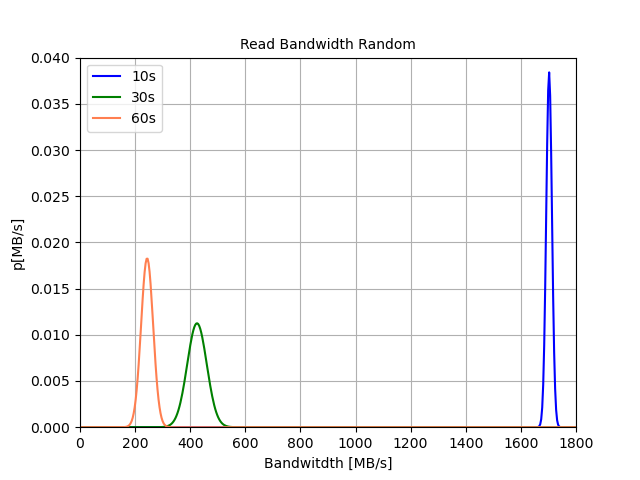
\includegraphics[width=\imgScale\textwidth]{Read_Bandwidth_Rand.png}}
                    \caption{Normal distribution of the readspeed for three different tests}
                    \label{fig:read-speed}
                \end{figure}   

                The read spead starts at around 1700MB/s, which is multiple times more than the other more saturated tests were able to achieve. 
                Considered the hardware architecture of the cluster, this value is only really achievable with caching data within the RAM.
                In fact the hardware requirements for a CEPH-Cluster demand around 2GB of RAM per OSD\textbf{REFERENCE HERE}.

                \begin{figure}[H]
                    \centering
                    \fbox{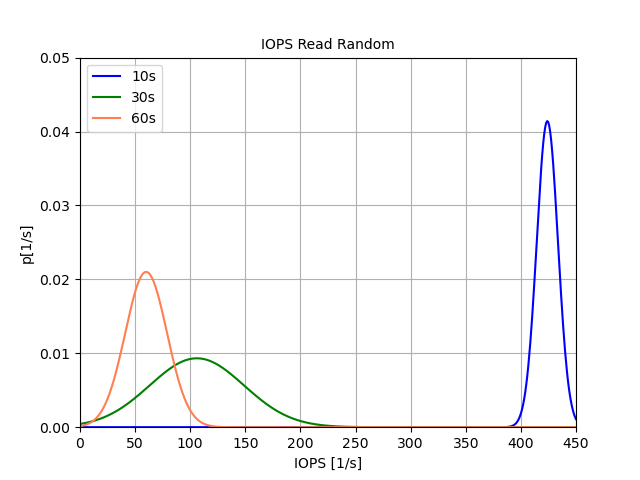
\includegraphics[width=\imgScale\textwidth]{Read_IOPS_Rand.png}}
                    \caption{Normal distribution of the read IOPS for three different tests}
                    \label{fig:read-iops}
                \end{figure}   

                The IOPS paint the same picture: very high cluster speed on the first few seconds with a more stabilized value after saturation of the caching chain. An interesting point is the high standard deviation before everything becomes saturated. I presume that it is the timespan, where
                some disks cache is already saturated and other caches are still filling up. Also the CPU of the host machine has only four logical cores and therefore quickly becomes task-saturated. The other cores in the cluster aren't that fast either. This results in the value stabilizing after around a minute.

                \begin{figure}[H]
                    \centering
                    \fbox{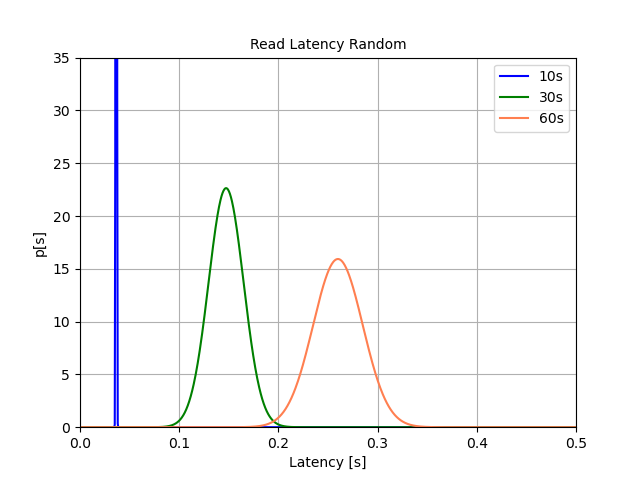
\includegraphics[width=\imgScale\textwidth]{Read_Latency_Random.png}}
                    \caption{Normal distribution of the read latency for three different tests}
                    \label{fig:read-latency}
                \end{figure}  

                The very fast response in the first ten seconds is the best argument that the data actually is read from the RAM instead 
                of the disks. The very small standard deviation can't really be achieved with different kinds of disks on iSCSI hosts. Referring to figure \ref*{fig:write-latency}, it is likely the same mechanic of reorganizing placement groups and data objects within the cluster which leads to increased latency. Also in conjunction with task saturation of the host machine.

            \subsection{Mysqlslap}\label{mysqlslap}

                The second test was a dedicatated load test specifically for SQL-Database\footnote{Although I used mySQL in this example, this applies also to other SQL-Based Database distributions.} workloads. The \textit{mysqlslap} application allows for some configuration on how the test is carried out:

                \begin{itemize}
                    \item Concurrent users
                    \item Iterations
                    \item Size and structure of automatically generated database table
                    \item Total number of queries
                \end{itemize}

                I load tested the database on three different storage technologies to point out potential advanteages and disadvantages of ceph in contrast to a purely HDD and SSD based storage solution - both were discrete disks in this example. The mySQL-Server was running on a VM\footnote{Virtual Machine} with the CentOS8 distribution.
                The VM ran on a physically seperate machine, which had the storage mounted by either NFS\footnote{Network File Storage} or the ceph kernel-module. The HDD and SSD based load test was carried out using the official mySQL-Docker Image\textbf{INSERT LINK TO DOCKER HUB}, because the configuration of different volumes is fairly unproblematic. This didn't work with the ceph kernel module for different reasons which I was unable to resolve entirely. Therefore the load test on ceph as the underlying storage was carried out using the native mySQL distribution for CentOS.

                To carry out the load test, I wrote the following script:

                \begin{lstlisting}
                    #!/bin/bash

                    ## db connection
                    dbuser=<mysql-user>
                    dbhost=127.0.0.1
                    dbpass=<mysql-password>

                    ## db test config
                    intcols=5
                    charcols=20

                    ## iterations over concurrent users
                    user_min=4
                    user_max=20
                    iterations=3
                    samples=5

                    ## queries per perfomance batch
                    total_queries=1024

                    for ((s=0; s<$samples; s++)) do
                        echo "Starting Sample number: $s"

                        for (( i=$user_min; i<=user_max; i++)) do
                            
                            queries_corrected=$((total_queries + (total_queries % $i)))
                            mysqlslap --user=$dbuser --host=$dbhost  --password=$dbpass --concurrency=$i --iterations=$iterations --number-int-cols=$intcols --number-char-cols=$charcols --number-of-queries=$queries_corrected --auto-generate-sql -v

                        done
                    done

                    exit 0
                \end{lstlisting}

                The core of the script is the \textit{mysqlslap} command being executed with different parametres.
                For the correct interpretation of the result I want to emphasize out a few key points:

                \paragraph{Single Threaded} operations of each user-session. The VM had four virtual cores, so a test with less than four concurrent user sessions doesn't yield any better or worse results.

                \paragraph{queries\_corrected} is a variable, which uses the modulo operation to correct the total number of queries to be executed slightly in order to always have every user executing the same amount of queries and don't run into bottlenecks due to uneven load-distribution.

                \paragraph{Samples and Iterations} is how I configured the script to execute multiple executions of the same load test in order to average out possible outliers. Each iteration is the same number depicted by \textit{total\_queries} n-times within the same \textit{mysqlslap} command. Each sample is the repetition of the 4-20 users cycle with three iterations each. This means, the same load test is carried out 15 times for each concurrent user setting.

                \begin{figure}[H]
                    \centering
                    \fbox{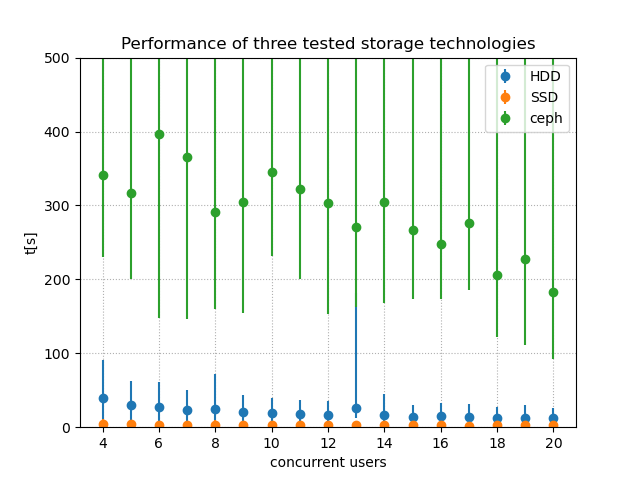
\includegraphics[width=\imgScale\textwidth]{mysqlslap.png}}
                    \caption{mySQL load test comparison between ceph/HDD/SSD}
                    \label{fig:mysql-loadtest}
                \end{figure}   

                The horizontal axis is concurrent users and the vertical scale the seconds until all 2048 queries were completed in average with the minimum and maximum time. The exact results of this test are made available in the Github repository\textbf{PUT GH LINK HERE}. By far the best performance was yielded by the SSD-based storage. There is a slight increase in perfomance with more concurrent users, since with a low session count neither the network interface nor the SSD and client machine has reached a bottleneck yet.
                At around 9-10 concurrent user sessions, the optimal performace is reached and declines slightly with more sessions. However due to the almost instantaneous nature of data access on SSDs, the major part of that time will be network roundtrip times, which add up over many queries.

                The same behaviour but much more distinct is shown by the HDD based storage. Since these drives have a measureable access time, this adds up to a more distinct increase of performance with increasing concurrency.
                This will likely be caused by optimizations in the access patterns of the physical disk. I do not have an explanation for the anomaly at the 13 user mark. Since even the minimum time is such an outlier compared to the 12 and 14 user mark, this can't be explained by some random occuring system-behaviour.

                The test of the ceph storage didn't turn out as expected. In fact the time to finish all queries was longer by one magnitudes in comparison to the HDD and two magnitude in case of the SSD.
                I have a few possible explanations for this behaviour and I think every one of these factors contributed at least partially:
                
                \paragraph{No NAT Reflection} The Docker macvlan network creates a virtual mac-adress for each container. However, it does not support NAT-Reflection, which results in every packet being routed to the central switch and back to the same physical host, which adds a lot of round-trip-time to the whole process.

                \paragraph{IOWAIT bottleneck} During the load test I watched the behaviour of the kernel of the docker-host and it showed that a significant portion - about 1/2 of the total CPU-time was allocated to IOWAIT processes. This indicates that communications with devices and interfaces are very slow. As to where this bottleneck is I could not find a definitive answer. My guess is that the sheer amount of virtual disks in conjunction with a high number of OSDs and the fact, that a few of them were iSCSI caused significant communication overhead, which adds up quickly in this situation.

                \paragraph{Missing OSD Network} As I explained in section \textbf{ARCHITECTURE LINK}, my setup doesn't have a dedicated network for the OSD traffic. It is possible that by using the same interface for server-client and OSD-OSD communication resulted in saturating the network interface, which isn't particularly high performance either. This is also a a good explanation for the IOWAIT kernel phenomenon.

                \paragraph{Slow disks} I used USB pen drives on the ARMv7 host, which were exported as iSCSI devices. I is possible that they degraded due to the heavy read and write load under the constant load and therefore decreased drastically in performace.

            \subsection{Disk Failure}

                One of my research goals defined in section\ref*{research-goal} was to examine the data integrity for database applications. During a dedicated loadtest I created a simulated drive failure by marking one or more OSDs as \textit{out}. This triggers a redistribution and replication of affected data objects as well as a change of the PG-Mapping. Ceph handled this process transparent for the client without any data loss.

                The MGR-Node creates an output of the cluster state, where the state of the placement groups is logged:

                \begin{lstlisting}
                    1 undersized+peered, 3 active+undersized, 42 active+clean, 7 active+clean+laggy, 7 stale+active+clean, 20 peering, 5 undersized+degraded+peered, 12 active+undersized+degraded; 1.1 GiB data, 7.0 GiB used, 27 GiB / 34 GiB avail; 9.6 MiB/s wr, 2 op/s; 105/1119 objects degraded (9.383%)
                \end{lstlisting}

                This is an example log output showing the status of a degraded and recovering cluster.
                Each unit depicts a placement group. \textbf{Active+Clean} is the desired state, whereas \textbf{stale} depicts an unresponsive pg. This could be network issues or a failed host, like in this case. If the log shows \textbf{peering}, it is undergoing the process of recovering the \textbf{degraded} data objects. During this process some pg's might have the temporary state of \textbf{active+undersized}, when the data shuffling is not yet complete and imbalances between the disks are existing. This is shown in the ceph OSD overview:

                \begin{lstlisting}
                    ceph osd df tree
                \end{lstlisting}

                brings up a general overview of the OSD status, which can be viewed here\textbf{PUT IN GITHUB HERE}. Interesting is the last line:

                \begin{lstlisting}
                    MIN/MAX VAR: 0.66/1.36  STDDEV: 6.22
                \end{lstlisting}

                This shows the imbalance of the pg placement on the different disks. The cluster could be configured to prefer certain disks for certain pgs, as with the metadata pool.

                \paragraph{Concluding} Ceph handles failure of disks gracefully and transparent as long as the failure can be contained and not too many disks fail. With a failed disk, the cluster will eventually reach a stable state after some time, when the data objects are rearranged on the disks. For databases this resulsts in reduced I/O performance but protects from data failures.

    \section{Conclusion}\label{conclusion}

        In this section I want to summarize the advantages and disadvantages of running a ceph-cluster by means of a containerized daemon structure.

        \subsection{Advantages}

            \paragraph{Ease of configuration} Once I figured out how to set up the OSDs and other daemons, it is fairly straighforward to set up a working cluster. I managed to compress this process into a single script\textbf{GH LINK HERE PLS}. The vanilla docker image is already configured in a way, which doesn't require extensive configuration beyond specifying the container parametres and preparing the disks.

            \paragraph{Orchestration} by using containers, the cluster could potentially be controlled on a higher level by means of orchestration tools such as \textit{kubernetes} or \textit{docker-swarm}. There also exists several solutions to abstract the cluster management: \textit{ceph-ansible} and \textit{rook}. \textbf{PUT REFERENCES HERE}. While reading through several issues on Github, it became clear, that these are used in production environments, which is a sign that these solutions are matured enough to be considered stable and performant.

            \paragraph{Updates} Since every container is stateless and ephemeral, the update process is in theory easier than an application running on bare metal. To update a container, it is sufficient to change the container-definition. However, how an upgrade of a whole cluster is carried out in general is beyond the scope of this paper.

            \paragraph{Shared KV-Backend} The docker image provides a way to use \textit{etcd} as a KV-storage\footnote{Key-Value} to share configurations and keyrings. This is handy to setup a cluster on multiple machines and distribute the cluster configuration automatically. This wasn't in the scope of my experiments, since all containers in my case were running on the same host and had access to the same harddrive.

            \paragraph{Multiple Daemons on the same host} In general it is not a problem to launch multiple MON, MGR, OSD and MDS containers on the same host. In fact, if orchestrated with kubernetes for example, it may happen if not explicitly specified otherwise that one worker-node\footnote{A host which runs kubernetes services}, hosts two or more monitor containers. However, as my test in section \ref{mysqlslap} clearly indicates, it is not recommended to run multiple OSD containers on the same host for reasons stated.

        \subsection{Disadvantages}

            \paragraph{Documentation} Although the Docker-Image has a fairly comprehensive documentation, I found that this approach is not very well documented in contrast to the usual \textit{bare-metal} usage of ceph. All official documentation are written on the assumption that the cluster is running directly on the host machine. Github Issues and Stackoverflow provide some degree of help but it is not comparable to the official ceph documentation by ceph and RedHat. An excpetion of this are the ready-to-use distributions with \textit{ceph-ansible} and \textit{rook}, which proofed to be helpflul in some cases.

            \paragraph{Performance} Although it should be obvious, it is clear that running such an application which relies on being "as-close" to the hardware as possible, comes with a perfomance penalty regardless of the degree of optimizations. If this really makes a huge difference on beefy machines is beyond the scope of this paper but should be taken into consideration nevertheless. 

            \paragraph{Persistence} As already explained in section \textbf{INSERT SECTIOON HERE}, containers are by principle ephemeral and stateless. Although persistent volumes and KV-Backends alleviate these properties for the most part, it creates some additional overhead, which wouldn't exist otherwise.

        \subsection{Performance}\label{performance:tuning}

            Although I was not able to compare the containerized solution to a cluster, which runs on \textit{bare-metal}, 
            the nature of containers allows for the educated guess that this solution at least will never be as performant. The extent of the difference however will depend on the machine, the cluster is running on. 

            There are several factors, which might have a bigger overall impact on the performance of the whole cluster, as I learned during the course of my reasearch. Optimize on these points might even be more effective in increasing performance such that the small performance penalty of running a containerized environment is worth the extra benefits. Possible optimizations could be:

            \paragraph{Running the MDS-Damon on fast SSD-based storage} Since the MDS only serves small but large amounts of data, it is totally feasable to use smaller but faster SSDs. Best performance would be reached by using modern nVME drives. Within the cluster configuration the placement groups for the metadata can be configured to be stored on these special drives. It is best practice to have a limited amount of users per any given MDS so there might even exist multiple sychronized copies of the same drive within the cluster to further improve performace.

            \paragraph{Use optimized Applications} Ceph does not only offer a filesystem, wich allows for the cluster to be used as virtual disk or block device but also libraries and API's to be directly implemented in clientside applications. The RedHat study\cite{redhatstudy} used an optimized mySQL distribution, which directly used the ceph kernel module to circumvent the filesystem bottleneck and yielded excellent results.

            \paragraph{Tune the cluster configuration} This might include tweaking the configuration for pool sizes, placement groups, stripe configs, object sizes and safety configuration such as crush map to the physical structure of the cluster in order to achieve best performance. The official ceph documentation provides extensive insight on how to do this.\textbf{INSERT REFERENCE HERE}

        \subsection{In Summary}

        To conclude my research goals pointed out in section \ref*{research-goal}, I found that like the study carried out by RedHat\cite{redhatstudy} a ceph cluster is well suited to be used as storage for a database in terms of data integrity. My test of removing OSDs during the mysql load test, showed that ceph handles failing disks in critical applications very well. However the fact that the OSDs are hosted within a containerized environment doesn't make a difference here. 
        
        I was not able to show a performance gain however for reasons stated in section \ref*{mysqlslap}.
        On the administion part I found that using containers drastically descreased the work neccessary to set up a cluster. However it cost me more work upfront to figure out the correct configuration. Therefore I'd conclude it does make sense for a huge production environment, where administion is a bigger concern than clusters which are set up once and subsequently aren't touched again as it is the case in smaller or mid-sized deployments.
      
    \bibliography{references}        
    \bibliographystyle{IEEEtran}

\end{document}